% !TeX root = Protokoll.tex
\begin{figure}
\subfloat{	
	\begin{adjustbox}{width=0.5\textwidth}
	\begin{tikzpicture}
			
			\node [draw=white, anchor=south west] (label) at (0,0) {
				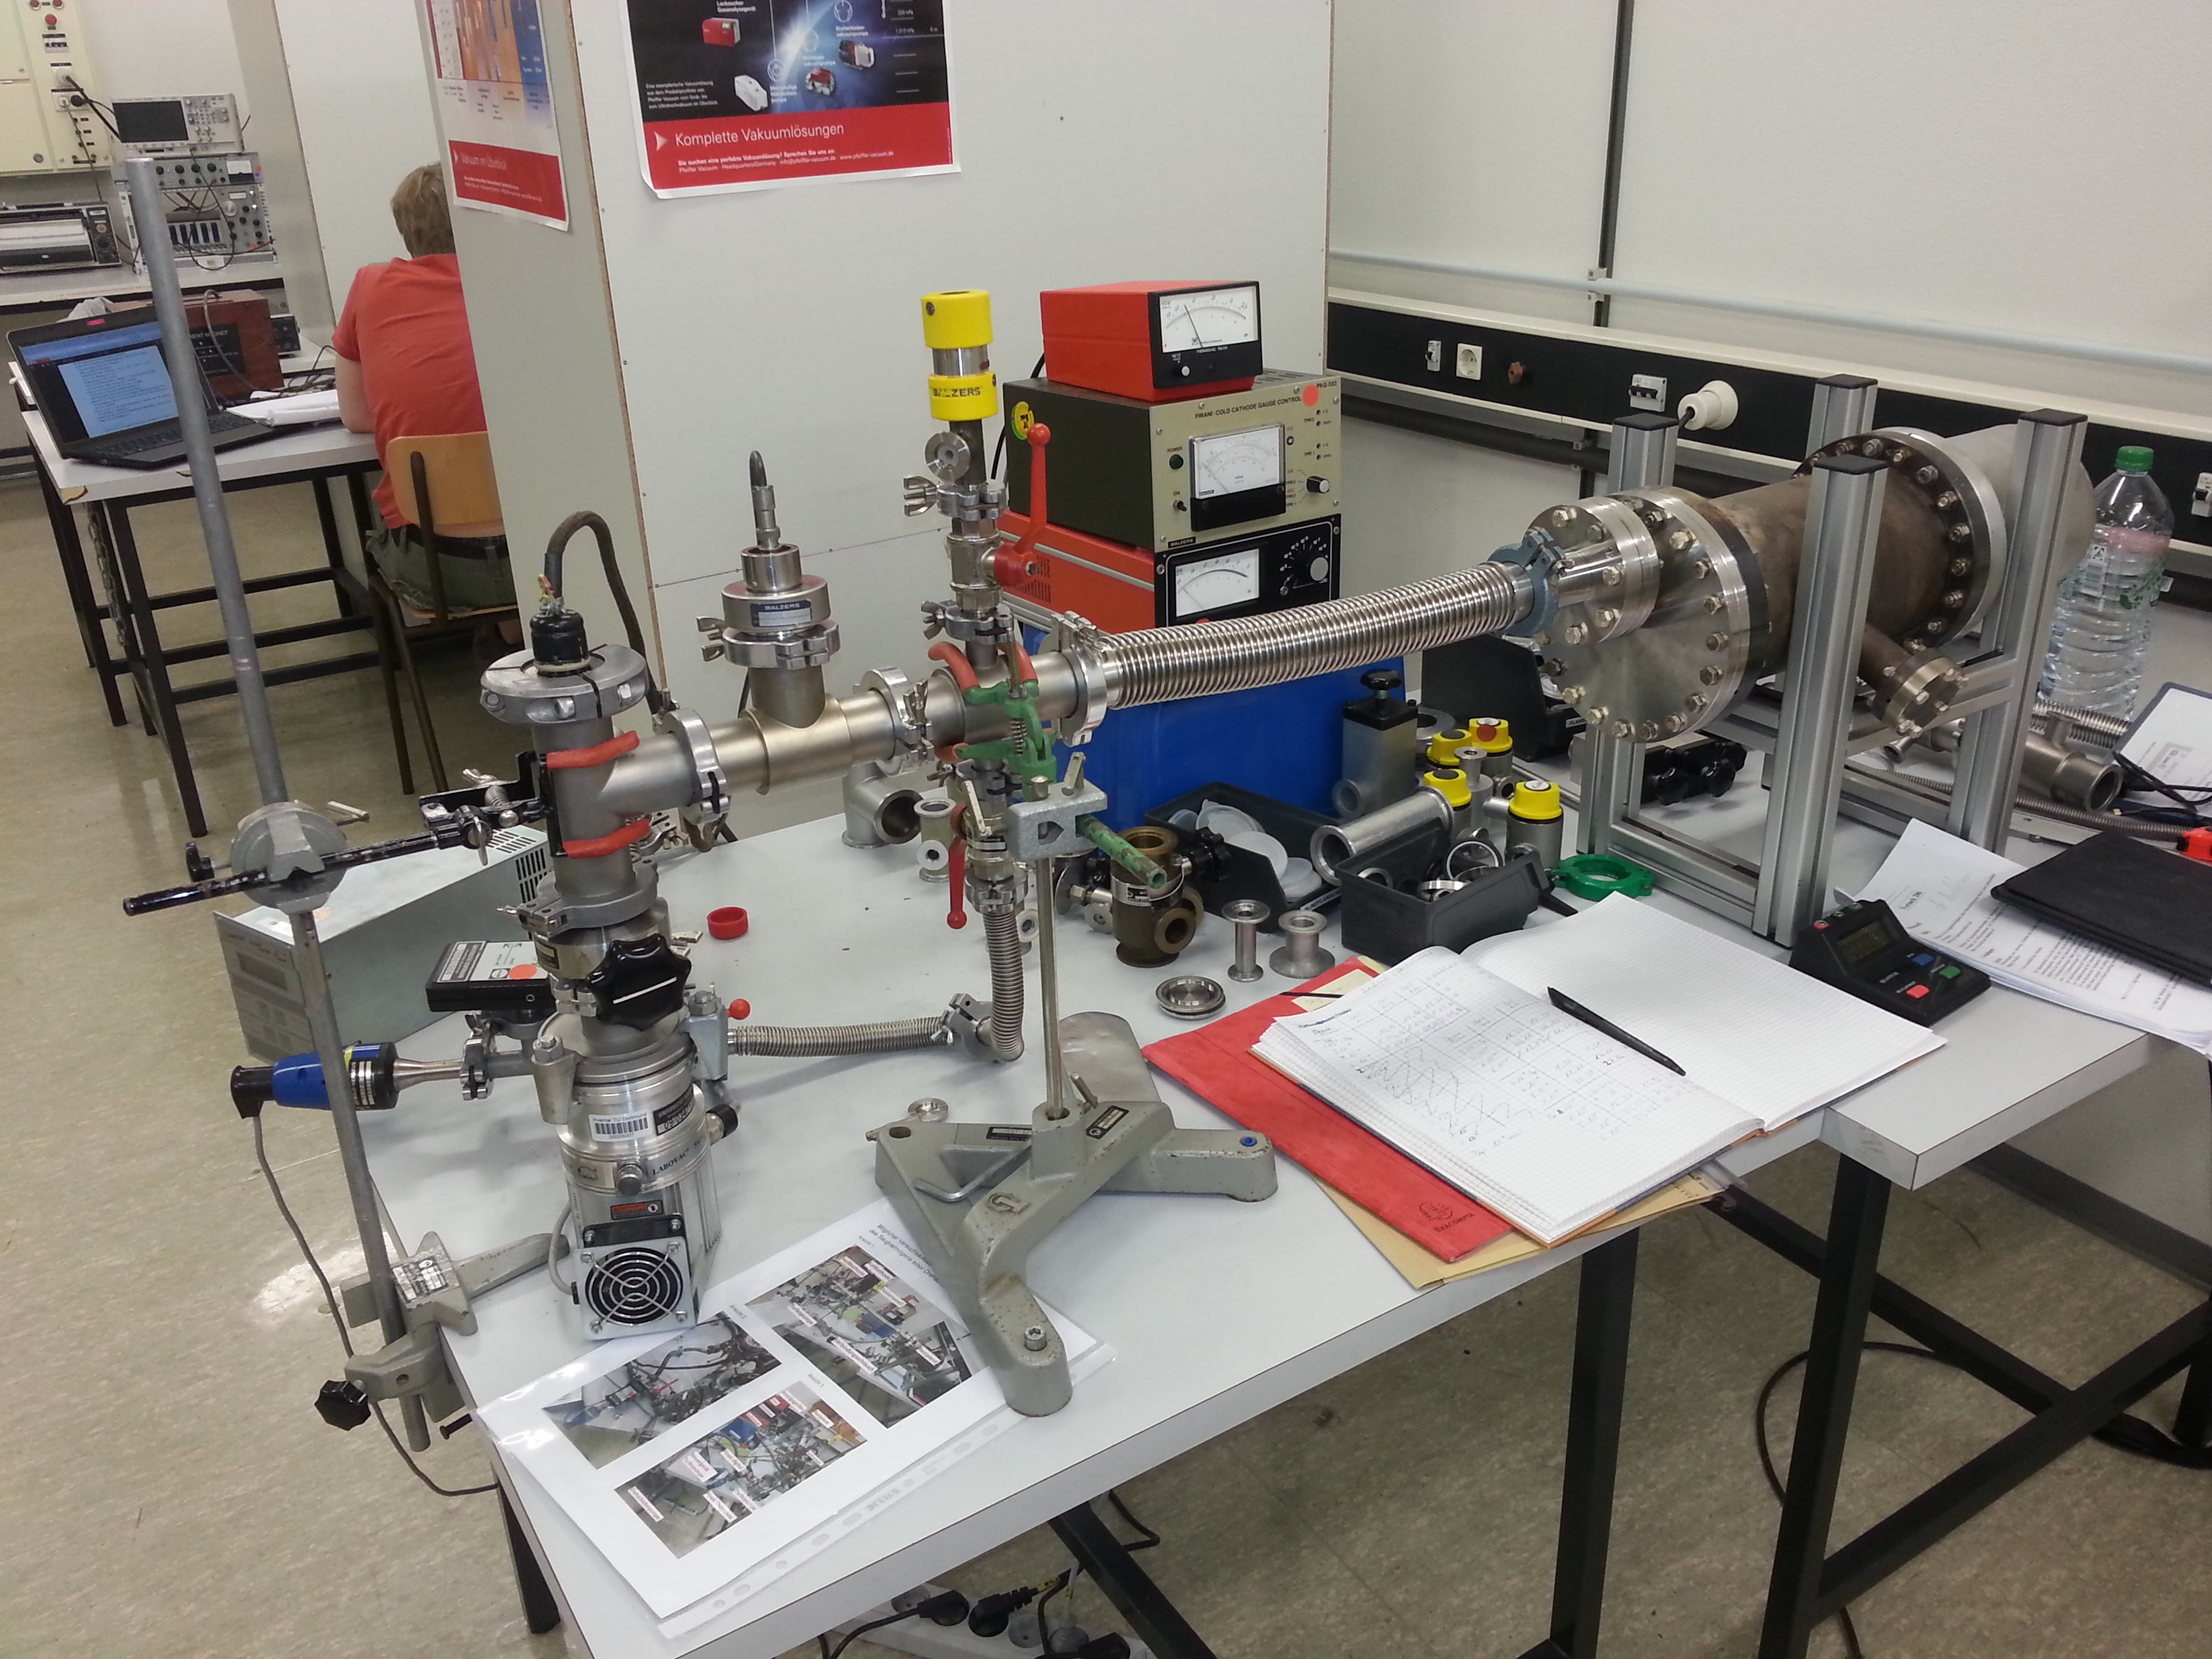
\includegraphics[width=\textwidth,scale=0.5]{../Grafiken/Aufbau.jpg}};
		%	\draw[step=.5cm,draw=gray] (0.15,0.15) grid (\textwidth,\textwidth - 110);
		%	\filldraw [fill=gray] (0.15,0.15) circle (1mm);
%			\foreach \x in {0,2,4,6,8,10,12,14,16}
%				\filldraw [fill=green] (\x,0) circle (2mm);
%			\foreach \y in {0,2,4,6,8,10,12}
%				\filldraw [fill=green] (0,\y) circle (2mm);
			
			\draw [thick] (15.0,10.65) -- (15.0,9.2);
			\node [draw=black,shape=circle,fill=lightgray] (1.) at (15.0,11) {1.3};
			
			\draw [thick] (13.75,9.65) -- (13.75,9);
			\node [draw=black,shape=circle,fill=lightgray] (1.) at (13.75,10) {1.2};
			

			
			\draw [thick] (14,8.15) -- (14,7.35);
			\node [draw=black,shape=circle,fill=lightgray] (1.) at (14,8.5) {1.3};
			
			\draw [thick] (12,9.15) -- (12,8.5);
			\node [draw=black,shape=circle,fill=lightgray] (1.) at (12,9.5) {1.4};
			
			\draw [thick] (10,8.15) -- (10,7.5);
			\node [draw=black,shape=circle,fill=lightgray] (2) at (10,8.5) {2};
			
			\draw [thick] (8.5,6.0) -- (7.5,7.0);
			\node [draw=black,shape=circle,fill=lightgray] (1) at (8.5,6.0) {9};
			
			\draw [thick] (8.5,8.0) -- (7.5,8.0);
			\node [draw=black,shape=circle,fill=lightgray] (1) at (8.5,8.0) {11};
			
			\draw [thick] (8.25,5)-- (7.25,6);
			\node [draw=black,shape=circle,fill=lightgray] (1) at (8.25,5) {11};
			
			\draw [thick] (6.0,5.5)-- (6.0,4.65);
			\draw [thick] (6.0,5.5)-- (7.4,5.10);
			\node [draw=black,shape=circle,fill=lightgray] (1) at (6.0,5.5) {3};
			
			\draw [thick] (6.5,8.5) -- (6,7.0);
			\node [draw=black,shape=circle,fill=lightgray] (2) at (6.5,8.5) {6};

			\draw [thick] (3.5,6.5) -- (4.5,6.5);
			\node [draw=black,shape=circle,fill=lightgray] (2) at (3.5,6.5) {8};
			
			\draw [thick] (3.5,5.25) -- (4.5,5.25);
			\node [draw=black,shape=circle,fill=lightgray] (2) at (3.5,5.25) {12};		

			\draw [thick] (3.5,4.25) -- (4.5,4.75);
			\node [draw=black,shape=circle,fill=lightgray] (2) at (3.5,4.25) {5};		
			
		\end{tikzpicture}
		\end{adjustbox}
}
\subfloat{
		\begin{adjustbox}{width=0.5\textwidth}
		\begin{tikzpicture}
		
		\node [draw=white, anchor=south west] (label) at (0,0) {
			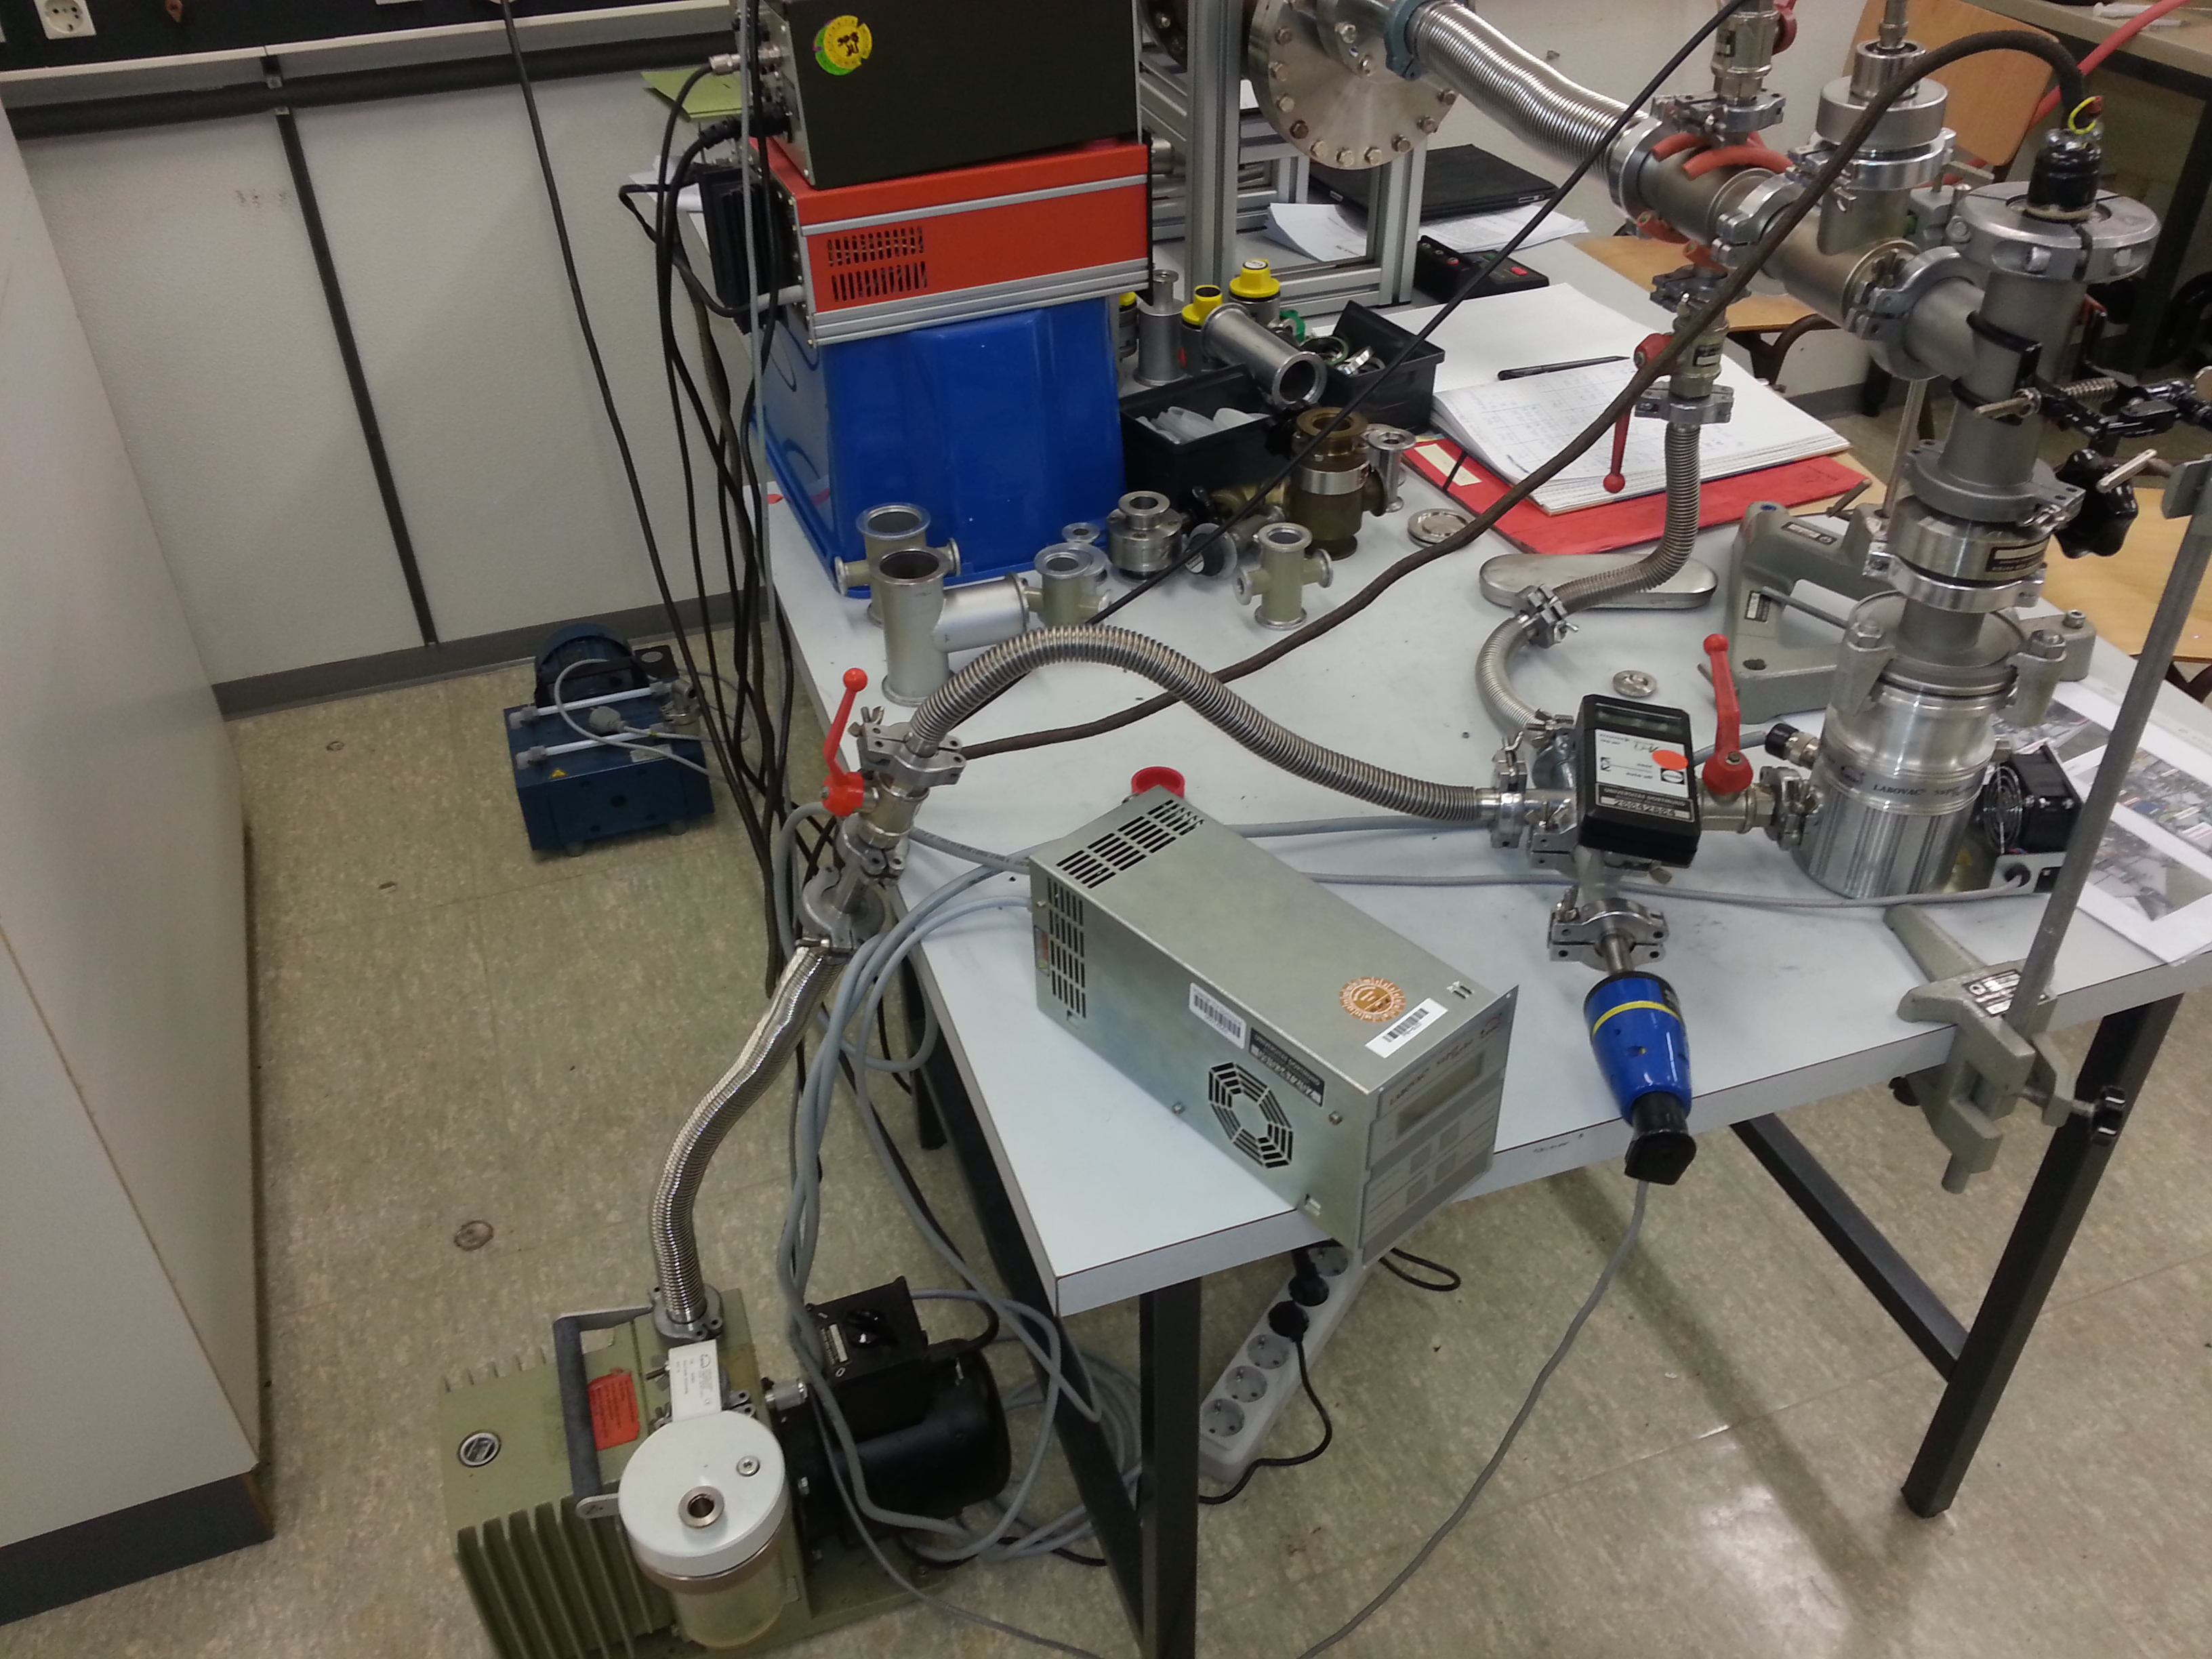
\includegraphics[width=\textwidth]{../Grafiken/Drehschieber.jpg}};
		%	\draw[step=.5cm,draw=gray] (0.15,0.15) grid (\textwidth,\textwidth - 110);
	%	\filldraw [fill=gray] (0.15,0.15) circle (1mm);
		%			\foreach \x in {0,2,4,6,8,10,12,14,16}
		%				\filldraw [fill=green] (\x,0) circle (2mm);
		%			\foreach \y in {0,2,4,6,8,10,12}
		%				\filldraw [fill=green] (0,\y) circle (2mm);
		
		\draw [thick] (12.5,8.) -- (12.5,6.5);
		\node [draw=black,shape=circle,fill=lightgray] (1.) at (12.5,8) {11};
		
		\draw [thick] (10.5,5.5) -- (11.5,6.35);
		\node [draw=black,shape=circle,fill=lightgray] (1.) at (10.5,5.5) {10};
				
		\draw [thick] (13,5.5) -- (11.75,5.85);
		\node [draw=black,shape=circle,fill=lightgray] (1.) at (13,5.5) {7};
		
		\draw [thick] (6.5,8.) -- (6.5,6.5);
		\node [draw=black,shape=circle,fill=lightgray] (1.) at (6.5,8) {11};
		
		\draw [thick] (8.,9.) -- (8.,7.5);
		\node [draw=black,shape=circle,fill=lightgray] (1.) at (8.,9) {4};

		\end{tikzpicture}
		\end{adjustbox}
	}
	\caption{Versuchsaufbau mit Nummerierung der Bauteile in \cref{tab:Bauteile_Abmessungen} \label{fig:Bauteile_Abmessungen}}
\end{figure}
	